\documentclass[../main.tex]{subfiles}
\usepackage{hyperref}

\begin{document}
\section{Data}
The Toronto Emotional Speech Set (TESS) is a well-established dataset
designed for emotion recognition in speech. The dataset consists of 2,800
audio samples of 200 target words spoken in seven distinct emotions
(angry, disgust, fear, happy, pleasant, surprised, sad, and neutral)
by two actors: a younger adult female (YAF) and an older adult female (OAF).
This creates a balanced dataset with 400 samples per emotion and 1,400
samples per speaker. This balance is crucial for training unbiased models,
as it ensures equal representation of each emotional class.

Additionally, to enhance the robustness of the model, we apply audio-specific
data augmentation. Augmentations such as random pitch shifting and
time-stretching effectively expand our dataset by introducing slight variability
in existing data, in turn making our model less prone to overfitting 
\citep{Bhatlawande2024}. These protocols ensure model robustness, aiding us in 
our goal of building a truly useful and reliable voice-based emotion classifier.

\begin{figure}[h]
    \centering
    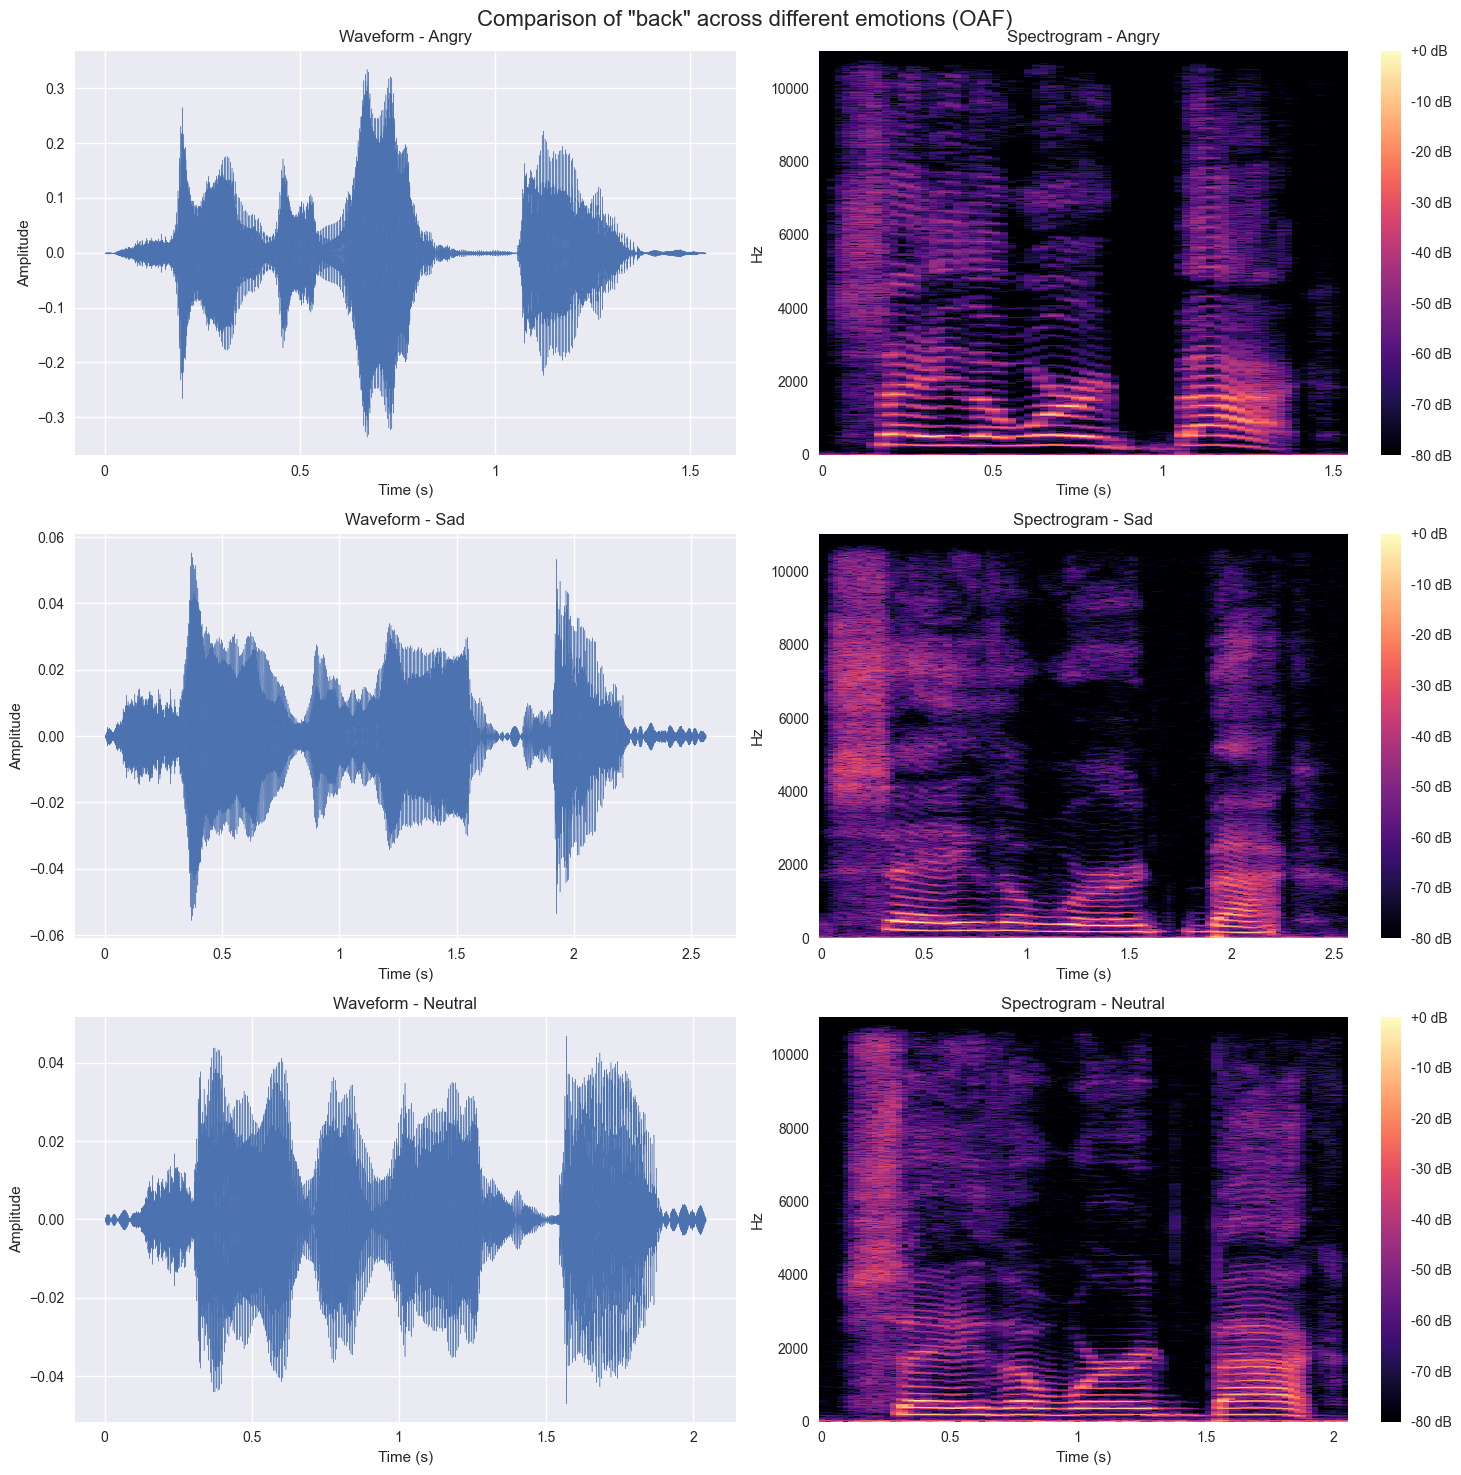
\includegraphics[width= 350pt]{../resources/tess_analysis.png}
    \caption{Comparison of waveforms and spectrograms of the word 
    ``back'' spoken with angry, sad, and neutral emotions by the older adult 
    female speaker (OAF). Left column shows the time-domain waveforms, the 
    right column shows the corresponding spectrograms with intensity in dB.}
    \label{fig:analysis}
\end{figure}

A key part of SER is extracting useful features from speech signals. The images shown 
in \autoref{fig:analysis} reveals several key patterns in how emotions 
affect speech characteristics. The waveforms show clear differences in amplitude, with
angry speech having the highest amplitude ($\pm$0.3), while sad and neutral speech
show much lower amplitudes ($\pm$0.06 and $\pm$0.04 respectively). In the spectrograms,
we can observe that angry speech displays more intense energy
(shown by brighter colors) especially in the 0-5 kHz range, while sad and
neutral expressions show more diffused energy patterns.

The temporal characteristics also vary notably across emotions. As seen in the
time axes, the sad utterance is the longest (around 2.5 seconds), while the
angry utterance is more compact (1.5 seconds), and the neutral utterance takes
a moderate duration (2 seconds). Looking at the spectrograms' frequency
distribution, angry speech shows distinct, high-intensity patterns
(visible as bright red-purple regions), whereas sad and neutral expressions
share similar, more subtle spectral patterns. These acoustic similarities
between certain emotion pairs, combined with varying temporal patterns,
suggest our model will need to consider both timing and frequency
characteristics to effectively classify emotions.


\end{document}
